\subsection{Application: Smart Grid Forecasting and Energy Systems}

Electric-load forecasting is a strong Foundations application because the quality of a forecast depends as much on data splitting and feature construction as on the regression algorithm. Electricity demand is highly autocorrelated, strongly periodic, and sensitive to calendar effects. If future information leaks into lagged features or normalization, a forecasting model can appear substantially more accurate than it would be in deployment. The central machine-learning problem is therefore to construct a causal supervised-learning dataset from a time series and to evaluate it with a genuinely forward-looking split.

The application also illustrates why simple baselines matter. A sophisticated model is only useful if it improves on persistence, seasonal repetition, or a regularized linear forecast built from the same historical information. Comparing against a 24-hour persistence baseline is especially informative for household and grid demand because daily periodicity is strong. The comparison therefore emphasizes the foundational ideas of baseline selection, temporal validation, feature engineering, and error analysis rather than architecture novelty.

The reproduced experiment uses the UCI Individual Household Electric Power Consumption dataset. Minute-level active-power measurements are aggregated to hourly load, and only lagged information available before the forecast time is used as input. A chronological train/test split is maintained after lag construction so that the held-out interval occurs strictly after the training interval.

\\textbf{Objective:} The objective is to construct a causal one-step-ahead hourly load-forecasting benchmark and determine whether learned models improve on a strong 24-hour seasonal persistence baseline under a strictly chronological holdout.

\textbf{Problem:} The task is one-step-ahead hourly electricity-demand forecasting. For each hour, the model predicts active power using recent demand history and calendar variables. The engineering objective is to reduce forecast error relative to a seasonal persistence rule while preserving a validation protocol that matches operational forecasting.

\\textbf{Dataset:} The experiment uses the UCI Individual Household Electric Power Consumption dataset (repository identifier 235), containing more than two million one-minute measurements collected from a household in Sceaux, France, from December 2006 through November 2010. The experiment aggregates global active power to hourly means and uses the final approximately 18 months of hourly observations to keep the benchmark computationally compact while preserving daily and weekly seasonality.

\\textbf{Model:} Three forecasting baselines are compared. A 24-hour persistence model predicts the current hour from the same hour on the previous day. Ridge regression provides a regularized linear model over lagged demand and cyclical calendar features. A histogram-based gradient-boosting regressor supplies a nonlinear baseline that can capture interactions among recent load, daily seasonality, weekly seasonality, and the lagged rolling mean.

\\textbf{Method:} Each supervised example contains demand lags at 1, 24, and 168 hours, a rolling 24-hour mean computed only from past values, and sine/cosine encodings of hour of day and day of week. After removing rows made incomplete by lag construction, the first 80\% of observations are used for training and the final 20\% for testing. This chronological split prevents future demand from leaking into model fitting.

\\textbf{Metrics:} The principal metrics are mean absolute error (MAE), root-mean-square error (RMSE), and mean absolute percentage error (MAPE) on the chronological test interval, supplemented by hour-of-day RMSE diagnostics.  Mean absolute error, root-mean-square error, and mean absolute percentage error summarize held-out forecast quality. Figure~\ref{fig:ch1-smart-grid-forecasting} contains two diagnostics. Panel (a) compares observed hourly demand with the three model forecasts over the final seven days of the test interval. Panel (b) reports hour-of-day RMSE for the 24-hour persistence baseline and the nonlinear gradient-boosting model, revealing when daily periodicity is easiest or hardest to predict. Table~\ref{tab:ch1-smart-grid-benchmark} reports the aggregate metrics.

\begin{figure}[t]
\centering
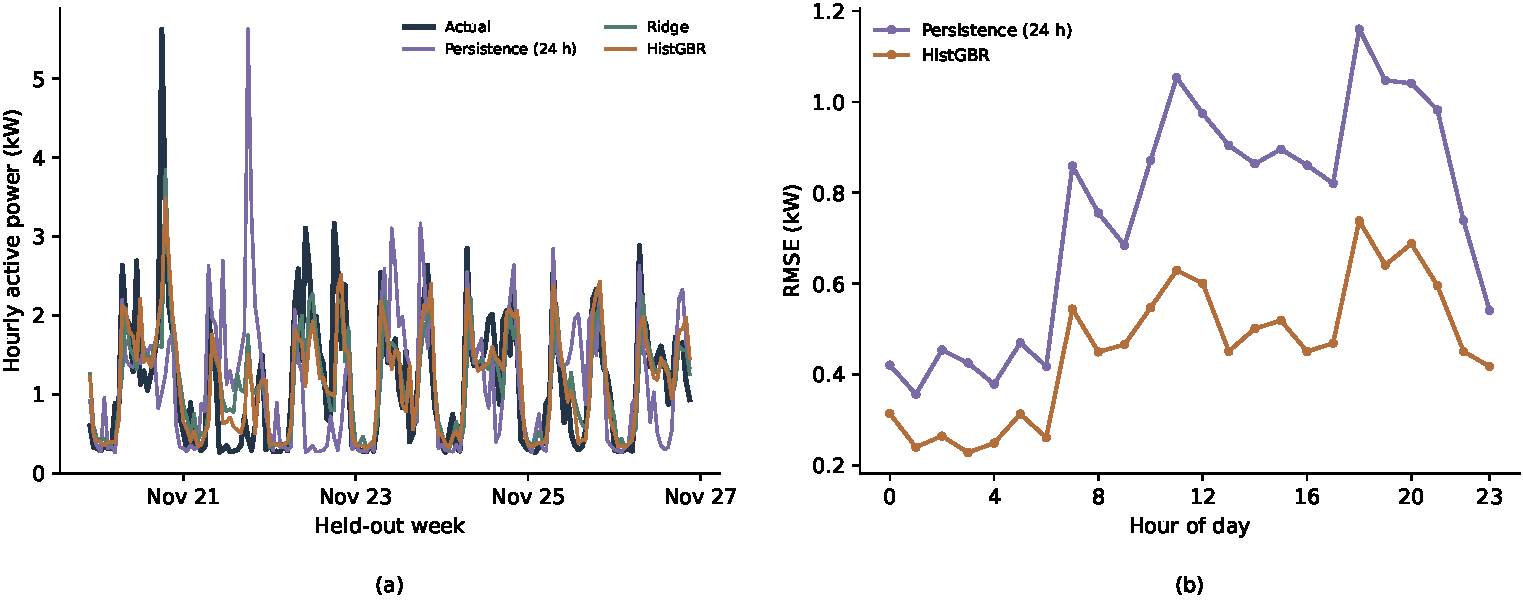
\includegraphics[width=\BookFigureWidth]{figures/ch01_smart_grid_load_forecasting.pdf}
\caption{Reproduced hourly electricity-load forecasting on the UCI Individual Household Electric Power Consumption dataset. (a) Actual hourly active power over the final seven days of the held-out interval compared with 24-hour persistence, ridge regression, and histogram gradient boosting. (b) Hour-of-day RMSE for persistence and gradient boosting, showing that forecast difficulty varies systematically across the daily load cycle. All features are constructed from information available before the prediction time, and the train/test split is chronological.}
\label{fig:ch1-smart-grid-forecasting}
\end{figure}

\begin{table}[t]
\centering
\small
\caption{Reproduced hourly load-forecasting benchmark using a chronological 80/20 split after lag construction. Lower values are better for all metrics.}
\label{tab:ch1-smart-grid-benchmark}
\begin{tabular}{lrrr}
\toprule
Model & MAE (kW) & RMSE (kW) & MAPE (\%) \\
\midrule
Persistence (24 h) & 0.5208 & 0.7888 & 65.39 \\
Ridge regression & 0.3754 & 0.5316 & 49.68 \\
Histogram gradient boosting & 0.3308 & 0.4825 & 43.35 \\
\bottomrule
\end{tabular}
\end{table}

\\textbf{Results:} Both learned models improve materially on the 24-hour persistence baseline under the same held-out interval. Ridge regression reduces RMSE from 0.7888 kW to 0.5316 kW, while histogram gradient boosting reduces it further to 0.4825 kW. The nonlinear model also achieves the lowest MAE and MAPE. The comparison shows the value of nonlinear interactions, but it also shows why a strong seasonal baseline is necessary: without persistence, the improvement would be difficult to interpret.

\\textbf{Error Analysis:} Forecast errors are not uniformly distributed through the day. Morning and evening demand transitions can be more difficult than stable overnight periods because load changes rapidly and daily routines vary. Residual analysis should therefore be stratified by hour of day, weekday versus weekend, season, and demand level. Large relative errors at low demand also explain why MAPE is much larger numerically than MAE or RMSE; this is a metric-property issue rather than evidence of an implementation error.

\\textbf{Limitations:} The dataset represents one household rather than a full transmission or distribution grid, and exogenous variables such as weather, price, holidays, and occupancy are not included in this controlled benchmark. The experiment therefore demonstrates foundational forecasting methodology rather than production-grade system forecasting. A utility-scale study should use multiple meters or substations, weather forecasts available at prediction time, rolling-origin backtesting, and uncertainty intervals.

\\textbf{Deployment / Engineering Implications:} The main Foundations lesson is that temporal validation determines whether a load forecast is credible. Random row splitting would leak future seasonal information and substantially weaken the deployment analogy. In production, the feature pipeline must guarantee causal lag construction, the model must be compared continuously with simple persistence baselines, and drift in load shape or seasonality should trigger recalibration or retraining.
